\documentclass[11pt,a4paper]{article}

\usepackage{amsmath,amssymb}
\usepackage{geometry}
\usepackage{booktabs}
\usepackage{xcolor}
\usepackage{listings}
\usepackage{tikz}
\usetikzlibrary{arrows.meta,calc,patterns}

\geometry{margin=2.5cm}

\definecolor{oldred}{RGB}{180,30,30}
\definecolor{newblue}{RGB}{20,80,160}
\definecolor{codegray}{RGB}{245,245,245}

\lstset{
  language=C++,
  basicstyle=\small\ttfamily,
  keywordstyle=\bfseries,
  commentstyle=\itshape\color{gray},
  backgroundcolor=\color{codegray},
  frame=single,
  framerule=0pt,
  xleftmargin=6pt,
  xrightmargin=6pt,
}

\title{%
  Transmissibility at Coarse--Fine LGR Interfaces\\[0.4em]
  \large What we had, what we have now}
\author{}
\date{\today}

% ================================================================
\begin{document}
\maketitle

% ----------------------------------------------------------------
\section{Notation}
% ----------------------------------------------------------------

\begin{center}
\begin{tabular}{cl}
\toprule
Symbol & Meaning \\
\midrule
$C$               & coarse cell adjacent to the LGR \\
$L$               & fine (LGR) cell sharing a face with $C$ \\
$\mathbf{x}_C$    & centroid of $C$ \\
$\mathbf{x}_L$    & centroid of $L$ \\
$F_C$             & the full face of $C$ that borders the LGR
                    (the \emph{parent face}) \\
$F_L$             & the face of $L$ that borders $C$
                    (a \emph{sub-face} of $F_C$) \\
$\mathbf{x}_{F_C}$& centre of the parent face $F_C$ \\
$\mathbf{x}_{F_L}$& centre of the sub-face $F_L$ \\
$A_L$             & area of the sub-face $F_L$ \\
$\hat{\mathbf{n}}$& unit outward normal to the face
                    (same direction for $F_C$ and $F_L$) \\
$k_C,\,k_L$      & permeability of $C$ and $L$
                    in the direction of $\hat{\mathbf{n}}$ \\
\bottomrule
\end{tabular}
\end{center}

\bigskip

When the LGR subdivides $F_C$ into $m$ sub-faces, each fine cell $L_i$
contributes one sub-face $F_{L_i}$ with centre $\mathbf{x}_{F_{L_i}}$.
The centres $\mathbf{x}_{F_{L_i}}$ are laterally \emph{offset} from
$\mathbf{x}_{F_C}$; the parent face centre $\mathbf{x}_{F_C}$ is their
common geometric mean only for a uniform subdivision.

% ----------------------------------------------------------------
\section{The TPFA half-transmissibility formula}
% ----------------------------------------------------------------

For any cell--face pair the TPFA half-transmissibility is
\begin{equation}
  T_{\text{half}} = k\;\frac{A\;|\mathbf{d}\cdot\hat{\mathbf{n}}|}{|\mathbf{d}|^{2}},
  \label{eq:halftrans}
\end{equation}
where $\mathbf{d}$ is the vector from the cell centroid to the face
centre used in the computation.

Write $\mathbf{d} = d_\perp\,\hat{\mathbf{n}} + \mathbf{d}_\parallel$,
where $d_\perp = \mathbf{d}\cdot\hat{\mathbf{n}}$ is the perpendicular
component and $\mathbf{d}_\parallel$ is the in-plane (tangential)
component.  Then
\begin{equation}
  T_{\text{half}} = k\;\frac{A\;|d_\perp|}{d_\perp^2 + |\mathbf{d}_\parallel|^2}.
  \label{eq:halftrans_decomp}
\end{equation}
When $\mathbf{d}_\parallel = \mathbf{0}$ this reduces to
the K-orthogonal formula $T_{\text{half}} = k\,A/|d_\perp|$.
When $|\mathbf{d}_\parallel| \gg |d_\perp|$ the denominator is dominated
by the tangential term and $T_{\text{half}}$ is strongly suppressed.

The interface transmissibility is the harmonic mean of the two sides:
\begin{equation}
  T_{CL} = \left(\frac{1}{T_{\text{half},C}} + \frac{1}{T_{\text{half},L}}\right)^{-1}.
\end{equation}

% ----------------------------------------------------------------
\section{Geometry at the coarse--fine interface}
% ----------------------------------------------------------------

\begin{center}
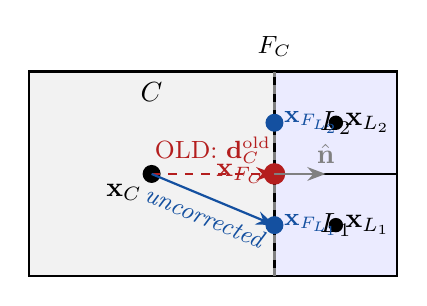
\begin{tikzpicture}[scale=1.3]
  % Coarse cell
  \fill[gray!10] (0,0) rectangle (2.4,2);
  \draw[thick] (0,0) rectangle (2.4,2);
  \node at (1.2,1.8) {$C$};

  % Fine cells
  \fill[blue!8] (2.4,0) rectangle (3.6,1);
  \fill[blue!8] (2.4,1) rectangle (3.6,2);
  \draw[thick] (2.4,0) rectangle (3.6,1);
  \draw[thick] (2.4,1) rectangle (3.6,2);
  \node at (3.0,0.5) {$L_1$};
  \node at (3.0,1.5) {$L_2$};

  % Centroids
  \fill[black] (1.2,1.0) circle (2.5pt);
  \node[below left] at (1.2,1.0) {$\mathbf{x}_C$};

  \fill[black] (3.0,0.5) circle (2pt);
  \node[right] at (3.0,0.5) {$\mathbf{x}_{L_1}$};
  \fill[black] (3.0,1.5) circle (2pt);
  \node[right] at (3.0,1.5) {$\mathbf{x}_{L_2}$};

  % Parent face F_C (dashed line)
  \draw[thick,dashed,gray] (2.4,0) -- (2.4,2);
  \node[above] at (2.4,2.05) {\small $F_C$};

  % Parent face centre x_{F_C}
  \fill[oldred] (2.4,1.0) circle (3pt);
  \node[left,oldred] at (2.4,1.0) {$\mathbf{x}_{F_C}$};

  % Sub-face centres x_{F_L1}, x_{F_L2}
  \fill[newblue] (2.4,0.5) circle (2.5pt);
  \node[right,newblue,font=\small] at (2.4,0.5) {$\mathbf{x}_{F_{L_1}}$};
  \fill[newblue] (2.4,1.5) circle (2.5pt);
  \node[right,newblue,font=\small] at (2.4,1.5) {$\mathbf{x}_{F_{L_2}}$};

  % Sub-face dividing line
  \draw[thick] (2.4,1) -- (3.6,1);

  % Normal arrow
  \draw[-{Stealth},thick,gray] (2.4,1.0) -- (2.9,1.0)
    node[above,gray] {$\hat{\mathbf{n}}$};

  % Distance vectors
  \draw[-{Stealth},thick,oldred,dashed]
    (1.2,1.0) -- (2.4,1.0)
    node[midway,above,oldred] {\small OLD: $\mathbf{d}_C^{\text{old}}$};
  \draw[-{Stealth},thick,newblue]
    (1.2,1.0) -- (2.4,0.5)
    node[midway,below,newblue,sloped] {\small \textit{uncorrected}};
\end{tikzpicture}
\end{center}

\medskip\noindent
The coarse cell $C$ has \textbf{two} sub-face connections: $C$--$L_1$ and
$C$--$L_2$.  The sub-face centres $\mathbf{x}_{F_{L_1}}$ and
$\mathbf{x}_{F_{L_2}}$ are displaced vertically from the parent face
centre $\mathbf{x}_{F_C}$.

% ----------------------------------------------------------------
\section{What we had (original code)}
% ----------------------------------------------------------------

\subsection*{Distance vectors and half-transmissibilities}

The parent face centre $\mathbf{x}_{F_C}$ was used for the coarse cell,
regardless of which fine cell $L_i$ was being processed.  The fine cell
always used its own sub-face centre $\mathbf{x}_{F_L}$:
\begin{align}
  \mathbf{d}_C^{\text{old}} &= \mathbf{x}_{F_C} - \mathbf{x}_C, \\[4pt]
  \mathbf{d}_L              &= \mathbf{x}_{F_L} - \mathbf{x}_L.
\end{align}

The resulting half-transmissibilities were:
\begin{align}
  T_{\text{half},C}^{\text{old}}
    &= k_C\;\frac{A_L\;
       |(\mathbf{x}_{F_C}-\mathbf{x}_C)\cdot\hat{\mathbf{n}}|}
       {|\mathbf{x}_{F_C}-\mathbf{x}_C|^{2}},
  \label{eq:Told_C}\\[6pt]
  T_{\text{half},L}^{\text{old}}
    &= k_L\;\frac{A_L\;
       |(\mathbf{x}_{F_L}-\mathbf{x}_L)\cdot\hat{\mathbf{n}}|}
       {|\mathbf{x}_{F_L}-\mathbf{x}_L|^{2}}.
  \label{eq:Told_L}
\end{align}

\subsection*{Consequences}

\begin{itemize}
  \item On a \textbf{Cartesian grid}, $\mathbf{x}_{F_C}$ lies directly
        in front of $\mathbf{x}_C$ (the vector $\mathbf{d}_C^{\text{old}}$
        is perpendicular to the face), so \eqref{eq:Told_C} reduces to the
        K-orthogonal formula $T_{\text{half},C} = k_C A_L / |d_\perp|$
        and the result was correct.
  \item On a \textbf{non-Cartesian grid}, $\mathbf{x}_{F_C}$ is
        laterally displaced from $\mathbf{x}_C$, introducing a small
        tangential component.  Because this displacement is the same for
        all sub-faces, however, $T_{\text{half},C}$ was still the same
        for every $L_i$: the result was \textbf{correct but asymmetric}
        on irregular grids.
  \item The function \texttt{getParentIntersectionFromLgrBoundaryFace}
        was called to retrieve $\mathbf{x}_{F_C}$.
\end{itemize}

% ----------------------------------------------------------------
\section{An intermediate step: sub-face centre for both cells}
% ----------------------------------------------------------------

A natural correction is to use the actual sub-face centre for $C$ as
well, so both sides see the same shared face:
\begin{equation}
  \mathbf{d}_C^{\text{sf}} = \mathbf{x}_{F_L} - \mathbf{x}_C.
\end{equation}

This is geometrically consistent and fixed the asymmetry.  However, it
introduced a large tangential component
\begin{equation}
  \mathbf{d}_\parallel = \mathbf{x}_{F_L} - \mathbf{x}_{F_C},
\end{equation}
which is the lateral offset of the sub-face centre from the parent face
centre.  For a layered reservoir with $\Delta x \gg \Delta z$ and
I-direction LGR refinement this offset dominates the distance vector and
the penalty in \eqref{eq:halftrans_decomp} is severe (see
Section~\ref{sec:numbers}).

% ----------------------------------------------------------------
\section{What we have now (adopted code)}
\label{sec:new}
% ----------------------------------------------------------------

\subsection*{Distance vector for $C$}

\begin{enumerate}
  \item Compute the raw vector to the sub-face centre:
        $\mathbf{d}_C^{\text{sf}} = \mathbf{x}_{F_L} - \mathbf{x}_C$.
  \item Extract the perpendicular component:
        $d_\perp = \mathbf{d}_C^{\text{sf}} \cdot \hat{\mathbf{n}}$.
  \item Discard the tangential part; keep only:
        \begin{equation}
          \boxed{\mathbf{d}_C^{\text{new}} = d_\perp\,\hat{\mathbf{n}}.}
          \label{eq:dnew}
        \end{equation}
\end{enumerate}

Geometrically, $\mathbf{d}_C^{\text{new}}$ is the orthogonal projection
of $\mathbf{d}_C^{\text{sf}}$ onto $\hat{\mathbf{n}}$: it points straight
from $\mathbf{x}_C$ to the face plane, with no lateral deviation.

\subsection*{Distance vectors and half-transmissibilities}

Let $d_\perp = (\mathbf{x}_{F_L} - \mathbf{x}_C)\cdot\hat{\mathbf{n}}$
be the perpendicular distance from the coarse centroid to the face plane
(evaluated along the sub-face direction, but independent of which sub-face
since all sub-faces share the same plane).  Then:
\begin{align}
  \mathbf{d}_C^{\text{new}} &= d_\perp\,\hat{\mathbf{n}},
  \label{eq:dnew_C}\\[4pt]
  \mathbf{d}_L              &= \mathbf{x}_{F_L} - \mathbf{x}_L
  \quad\text{(unchanged)}.
  \label{eq:dnew_L}
\end{align}

The resulting half-transmissibilities are:
\begin{align}
  T_{\text{half},C}^{\text{new}}
    &= k_C\;\frac{A_L\;|d_\perp|}{|d_\perp|^2}
     = \frac{k_C\,A_L}{|d_\perp|}
     = \frac{k_C\,A_L}
            {|(\mathbf{x}_{F_L}-\mathbf{x}_C)\cdot\hat{\mathbf{n}}|},
  \label{eq:Tnew_C}\\[6pt]
  T_{\text{half},L}^{\text{new}}
    &= k_L\;\frac{A_L\;
       |(\mathbf{x}_{F_L}-\mathbf{x}_L)\cdot\hat{\mathbf{n}}|}
       {|\mathbf{x}_{F_L}-\mathbf{x}_L|^{2}}.
  \label{eq:Tnew_L}
\end{align}

\noindent
$T_{\text{half},L}^{\text{new}} = T_{\text{half},L}^{\text{old}}$:
the fine-cell formula is identical before and after.

\subsection*{Consequences}

\begin{itemize}
  \item $\mathbf{d}_C^{\text{new}}$ is perpendicular to the face by
        construction, so the K-orthogonal formula \eqref{eq:Tnew_C} is
        always recovered with no tangential penalty:
        \begin{equation*}
          T_{\text{half},C}^{\text{new}} = \frac{k_C\,A_L}{|d_\perp|}.
        \end{equation*}
  \item $d_\perp = \mathbf{d}_C^{\text{sf}}\cdot\hat{\mathbf{n}}$ is
        the same for every sub-face $F_{L_i}$ on the same parent face
        (they all lie on the same plane with the same normal), so
        $T_{\text{half},C}$ is identical for all $L_i$:
        \textbf{symmetry is guaranteed}.
  \item On a Cartesian grid $\mathbf{d}_C^{\text{new}}$ equals
        $\mathbf{d}_C^{\text{old}}$: no regression for regular grids.
  \item \texttt{getParentIntersectionFromLgrBoundaryFace} is no longer
        called.
\end{itemize}

% ----------------------------------------------------------------
\section{Comparison table}
% ----------------------------------------------------------------

\begin{center}
\begin{tabular}{lccc}
\toprule
 & \textbf{Old} & \textbf{Intermediate} & \textbf{New (adopted)} \\
\midrule
Face centre for $C$ &
  $\mathbf{x}_{F_C}$ &
  $\mathbf{x}_{F_L}$ &
  $\mathbf{x}_C + d_\perp\hat{\mathbf{n}}$ \\[4pt]
Face centre for $L$ &
  $\mathbf{x}_{F_L}$ &
  $\mathbf{x}_{F_L}$ &
  $\mathbf{x}_{F_L}$ \\[4pt]
$\mathbf{d}_\parallel = \mathbf{0}$ for $C$ &
  Cartesian only &
  Never &
  Always \\[4pt]
$T_{\text{half},C} = k_C A_L / |d_\perp|$ &
  Cartesian only &
  Never &
  Always \\[4pt]
Same $T_{\text{half},C}$ for all $L_i$ (symmetry) &
  Always &
  Always &
  Always \\[4pt]
Symmetry on non-Cartesian grids &
  \textcolor{oldred}{No} &
  \textcolor{newblue}{Yes} &
  \textcolor{newblue}{Yes} \\[4pt]
Mass conservation (no flow barrier) &
  \textcolor{newblue}{Yes} &
  \textcolor{oldred}{No (large $\Delta x/\Delta z$)} &
  \textcolor{newblue}{Yes} \\
\bottomrule
\end{tabular}
\end{center}

% ----------------------------------------------------------------
\section{Numerical example: HORIZONTAL-WELL-REFINED}
\label{sec:numbers}
% ----------------------------------------------------------------

Grid: $\Delta x = 300\,\text{m}$, $\Delta z = 25\,\text{m}$,
LGR with 2$\times$ I-refinement.

At the K-direction coarse--fine interface:
\begin{align*}
  d_\perp &= \tfrac{\Delta z}{2} = 12.5\,\text{m},\\
  |\mathbf{d}_\parallel^{\text{sf}}|
          &= \tfrac{\Delta x}{4} = 75\,\text{m}
           \quad\text{(lateral sub-face offset)}.
\end{align*}

\begin{center}
\begin{tabular}{lcc}
\toprule
 & $|\mathbf{d}_C|^2\;[\text{m}^2]$
 & $T_{\text{half},C}\,/\,(k_C A_L / d_\perp)$ \\
\midrule
Old code ($\mathbf{x}_{F_C}$, Cartesian grid)
  & $12.5^2 = 156$   & $1.000$ \\
Intermediate ($\mathbf{x}_{F_L}$, sub-face centre)
  & $12.5^2+75^2 = 5781$ & $0.027$ \\
New code (projection onto $\hat{\mathbf{n}}$)
  & $12.5^2 = 156$   & $1.000$ \\
\bottomrule
\end{tabular}
\end{center}

\medskip\noindent
The intermediate construction reduces $T_{\text{half},C}$ to $2.7\%$ of
the correct value because $\Delta x/\Delta z = 12$ and the sub-face
offset ($75\,\text{m}$) dominates the perpendicular distance
($12.5\,\text{m}$).  This creates a near-complete flow barrier at the
LGR boundary and is the source of the mass conservation failure.  The
new code recovers the full transmissibility.

% ----------------------------------------------------------------
\section{Code in terms of the notation above}
% ----------------------------------------------------------------

\paragraph{Old code.}
The coarse face centre was obtained from the parent intersection
(corresponding to $\mathbf{x}_{F_C}$); the fine cell used
\texttt{faceCenterEcl} (corresponding to $\mathbf{x}_{F_L}$).

\begin{lstlisting}
// x_{F_C}: centre of the full parent face
const auto& parentIntersection =
    grid_.getParentIntersectionFromLgrBoundaryFace(intersection);

inside.faceCenter  = (inside.level()  == 0)
    ? parentIntersection.geometry().center()            // x_{F_C}
    : grid_.faceCenterEcl(inside.elemIdx,  ...);        // x_{F_L}
outside.faceCenter = (outside.level() == 0)
    ? parentIntersection.geometry().center()            // x_{F_C}
    : grid_.faceCenterEcl(outside.elemIdx, ...);        // x_{F_L}
\end{lstlisting}

\paragraph{New code.}
Both cells start from the sub-face centre $\mathbf{x}_{F_L}$.  For the
coarse cell only, the tangential part of
$\mathbf{d}_C^{\text{sf}} = \mathbf{x}_{F_L} - \mathbf{x}_C$ is then
removed, leaving $\mathbf{d}_C^{\text{new}} = d_\perp\,\hat{\mathbf{n}}$.

\begin{lstlisting}
// Both start from x_{F_L} (actual sub-face centre)
inside.faceCenter  = grid_.faceCenterEcl(inside.elemIdx,  ...); // x_{F_L}
outside.faceCenter = grid_.faceCenterEcl(outside.elemIdx, ...); // x_{F_L}

const auto nhat = intersection.centerUnitOuterNormal(); // n-hat

// For the coarse cell: project faceCenter so that
//   d_C = faceCenter - x_C  becomes  d_perp * nhat
auto projectCoarseFaceCenter = [&](DimVector& faceCenter, unsigned idx) {
    const auto d = distanceVector_(faceCenter, idx); // d_C^sf = x_{F_L} - x_C
    const Scalar d_perp = Dune::dot(d, nhat);         // d_perp
    for (unsigned k = 0; k < dimWorld; ++k)
        faceCenter[k] -= d[k] - d_perp * nhat[k];    // remove d_parallel
    // now: faceCenter - x_C = d_perp * nhat  => d_C^new
};

if (intersection.inside().level() == 0)               // C is inside
    projectCoarseFaceCenter(inside.faceCenter,  inside.elemIdx);
else                                                   // C is outside
    projectCoarseFaceCenter(outside.faceCenter, outside.elemIdx);
\end{lstlisting}

\noindent
After \texttt{projectCoarseFaceCenter}, when \texttt{computeHalfTrans\_}
calls \texttt{distanceVector\_(faceCenter, x\_C)}, it receives
$\mathbf{d}_C^{\text{new}} = d_\perp\,\hat{\mathbf{n}}$, so
\eqref{eq:halftrans} gives
\begin{equation*}
  T_{\text{half},C}
    = k_C\;\frac{A_L\;|d_\perp|}{|d_\perp|^2}
    = \frac{k_C\,A_L}{|d_\perp|},
\end{equation*}
the correct K-orthogonal result.

\end{document}
